% bei Standalone in documentclass noch:
% \RequirePackage{luatex85}

\documentclass[captions=tableheading, titlepage= firstiscover, parskip = half , bibliography=totoc]{scrartcl}
%paper = a5 für andere optinen
% titlepage= firstiscover
% bibliography=totoc für bibdateien
% parskip=half  Veränderung um Absätze zu verbessern

\usepackage{scrhack} % nach \documentclass
\usepackage[aux]{rerunfilecheck}
\usepackage{polyglossia}
\usepackage[style=numeric, backend=biber]{biblatex} % mit [style = alphabetic oder numeric] nach polyglossia
\addbibresource{lit.bib}
\setmainlanguage{german}

\usepackage[autostyle]{csquotes}
\usepackage{amsmath} % unverzichtbare Mathe-Befehle
\usepackage{amssymb} % viele Mathe-Symbole
\usepackage{mathtools} % Erweiterungen für amsmath
\usepackage{fontspec} % nach amssymb
% muss ins document: \usefonttheme{professionalfonts} % für Beamer Präsentationen
\usepackage{longtable}

\usepackage[
math-style=ISO,    % \
bold-style=ISO,    % |
sans-style=italic, % | ISO-Standard folgen
nabla=upright,     % |
partial=upright,   % /
]{unicode-math} % "Does exactly what it says on the tin."
\setmathfont{Latin Modern Math}
% \setmathfont{Tex Gyre Pagella Math} % alternativ

\usepackage[
% die folgenden 3 nur einschalten bei documenten
locale=DE,
separate-uncertainty=true, % Immer Fehler mit ±
per-mode=symbol-or-fraction, % m/s im Text, sonst \frac
]{siunitx}

% alternativ:
% per-mode=reciprocal, % m s^{-1}
% output-decimal-marker=., % . statt , für Dezimalzahlen

\usepackage[
version=4,
math-greek=default,
text-greek=default,
]{mhchem}

\usepackage[section, below]{placeins}
\usepackage{caption} % Captions schöner machen
\usepackage{graphicx}
\usepackage{grffile}
\usepackage{subcaption}

% \usepackage{showframe} Wenn man die Ramen sehen will

\usepackage{float}
\floatplacement{figure}{htbp}
\floatplacement{table}{htbp}

\usepackage{mhchem} %chemische Symbole Beispiel: \ce{^{227}_{90}Th+}


\usepackage{booktabs}

 \usepackage{microtype}
 \usepackage{xfrac}

 \usepackage{expl3}
 \usepackage{xparse}

 % \ExplSyntaxOn
 % \NewDocumentComman \I {}  %Befehl\I definieren, keine Argumente
 % {
 %    \symup{i}              %Ergebnis von \I
 % }
 % \ExplSyntaxOff

 \usepackage{pdflscape}
 \usepackage{mleftright}

 % Mit dem mathtools-Befehl \DeclarePairedDelimiter können Befehle erzeugen werden,
 % die Symbole um Ausdrücke setzen.
 % \DeclarePairedDelimiter{\abs}{\lvert}{\rvert}
 % \DeclarePairedDelimiter{\norm}{\lVert}{\rVert}
 % in Mathe:
 %\abs{x} \abs*{\frac{1}{x}}
 %\norm{\symbf{y}}

 % Für Physik IV und Quantenmechanik
 \DeclarePairedDelimiter{\bra}{\langle}{\rvert}
 \DeclarePairedDelimiter{\ket}{\lvert}{\rangle}
 % <name> <#arguments> <left> <right> <body>
 \DeclarePairedDelimiterX{\braket}[2]{\langle}{\rangle}{
 #1 \delimsize| #2
 }

\setlength{\delimitershortfall}{-1sp}

 \usepackage{tikz}
 \usepackage{tikz-feynman}

 \usepackage{csvsimple}
 % Tabellen mit \csvautobooktabular{"file"}
 % muss in table umgebung gesetzt werden


% \multicolumn{#Spalten}{Ausrichtung}{Inhalt}

\usepackage{hyperref}
\usepackage{bookmark}
\usepackage[shortcuts]{extdash} %nach hyperref, bookmark

\newcommand{\ua}[1]{_\symup{#1}}
\newcommand{\su}[1]{\symup{#1}}

\title{Versuch 206}
\subtitle{Die Wärmepumpe}
\author{Jonah Nitschke\\
        lejonah@web.de \and
        Sebastian Pape\\
        sepa@gmx.de}
\date{Durchführung: 15.11.2016\\
      Abgabe: 22.11.2016}

\begin{document}

\maketitle
\tableofcontents
\newpage

\section{Einführung}

Im folgendem Versuch geht es um den Transport von Wärmeenergie zwischen zwei Wärmereservoiren.
Im Gegensatz zu der allgemein gültigen Regel, wird hier nun mithilfe einer Wärmepumpe
Wärmeenergie von einem Reservoir mit kaltem Wasser in ein Reservoir mit warmen Wasser transponiert.
Während des Versuchs werden verschiedene Messwerte aufgenommen, um hinterher das Verhältniss von Temperatur,
Druck sowie aufgewandter Arbeit zu beurteilen.

\section{Theorie}

% Einfügen von Kommentaren zur Thermodynamik aus blauer Mappe

Damit nun in dem folgendem Versuch der Wärmefluss von dem kälteren Reservoir zu dem
wärmeren Reservoir realisiert werden kann, muss zusätzliche Arbeit aufgewandt werden. Für diesen Prozess wird eine Wärmepumpe benutzt, deren Aufbau später noch in Kapitel 3 erläutet wird und deren Bedingungen
zur Vereinfachung der Berechnungen als idealisiert betrachtet werden.

Um das Verhältnis von transponierter Wärmemenge zu aufgewandter Arbeit anzugeben, wird die Güteziffer
$\nu$ eingeführt. Nach dem ersten Hauptsatz der Thermodynamik \eqref{eqn:1HSa} gilt für den Wärmenergietransport
zwischen zwei Medien:

\begin{align}
  \increment U &= \increment Q + \increment W \label{eqn:1HSa} \\
  Q_1          &= Q_2 + A   \label{eqn:1HSb}
\end{align}

Die in unserem Fall geltende 2. Formel \eqref{eqn:1HSb} sagt, dass die vom Transportmedium am Reservoir 2 abgegebene
Wärmeenergie $Q_1$, der Summe der aus Reservoir 1 entnommenen Wärmeenergie $Q_2$ und der aufgewandten Arbeit $A$
entsprechen muss. Die Güteziffer der Wärmepumpe kann somit über folgende Formel errechnet werden:

\begin{equation}
  \nu = \frac{Q1}{A}
\end{equation}

Nach dem 2.HS der Thermodynamik lässt sich zudem die Beziehung zwischend den Wärmemengen und Temperaturen der
beiden Reservoire durch folgende Formel ausdrücken:

\begin{equation}
  \label{eqn:2HS}
  \frac{Q_1}{T_1} - \frac{Q_2}{T_2} = 0
\end{equation}

Für die Gültigkeit dieser Formel muss jedoch gelten, dass der stattfindende Übertragungsprozess reversibel sei.
Somit müsste die aufgewandte mechanische Energie jederzeit vollständig zurückgewonnen werden können. Da es
sich dabei um eine idealisierte Annahme handelt, die in der Realität nie zutrifft, muss \eqref{eqn:2HS}
umformuliert werden:

\begin{equation}
  \label{eqn:2HS1}
  \frac{Q_1}{T_1} - \frac{Q_2}{T_2} > 0
\end{equation}

Aus den Gleichungen (1) bis (4) folgt somit:

\begin{align}
  \nu_{id}   &= \frac{Q_1}{A} = \frac{T_1}{T_1 - T_2} \label{eqn:A1.2} \\
  \nu_{real} &= \frac{Q_1}{A} < \frac{T_1}{T_1 - T_2} \label{eqn:A1.3}
\end{align}

Die Gleichungen \eqref{eqn:A1.2} und \eqref{eqn:A1.3} zeigen, dass eine Wärmepumpe umso effektiver eingestuft werden
kann, je kleiner die Differenz zwischen $T_1$ und $T_2$ ist.

\subsection{Bestimmung der realen Güteziffer \texorpdfstring{$\nu$}{z}}

Mit dem Werten von $T_1$ kann nun die pro Zeiteinheit gewonnene Wärmemenge berechnet werden:

\begin{align}
  \label{eqn:Gueteziffer}
  \frac{\increment Q_1}{\increment t} &= (m_1c_W + m_kc_k) \frac{\increment T_1}{\increment t} \\
  \label{eqn:Güte_theo}
  \nu                                 &= \frac{\increment Q_1}{\increment t N}
\end{align}

$m_1c_w$ und $m_kc_k$ entsprechen dabei den Wärmekapazitäten der Kupferschlange und des Eimers.
Für die Güteziffer wird noch $N$ als die zeitlich gemittelte Leistung benötigt.

\subsection{Bestimmung des Massendurchsatzes}

Mit den Werten von $T_2$ und der Verdampfungswärme $L$ kann nun der Massendurchsatz $\increment m $
berechnet werden:

\begin{align}
  \label{eqn:Massendurchsatz}
  \frac{\increment Q_2}{\increment t} &= (m_2 c_W + m_k c_k) \frac{\increment T_2}{\increment t} \\
  \label{eqn:Massendurchsatz1}
  \frac{\increment Q_2}{\increment t} &= L \frac{\increment m}{\increment t}
\end{align}

\subsection{Bestimmung der mechanischen Kompressorleistung \texorpdfstring{$N_{mech}$}{t} }

Um die mechnanische Kompressorleistung $N_{mech}$ zu bestimmen muss vorher die vom Kompressor aufgebrachte
Arbeit zur Komprimierung des Volumens $V_a$ auf das Volumen $V_b$ berechnet werden:

\begin{equation}
  \label{eqn:Am}
  A_m = \frac{1}{\kappa - 1} \left( p_b \sqrt[\kappa]{\frac{p_a}{p_b}} - p_a \right) V_a
\end{equation}

Für den Kompressor wird nun näherungsweise angenommen, dass es sich um eine adiabatische Komprimierung handelt,
sodass die Poisson-Gleichung als Zusammenhang zwischen Druck und Volumen gilt:

\begin{equation}
  p_a V^{\kappa}_a = p_b V^{\kappa}_b = p V^{\kappa} .
\end{equation}

Mit der Dichte $\rho$ im gasförmigen Zustand, also beim Druck $p_a$, kann nun $N_{mech}$ berechnet werden:

\begin{equation}
  \label{eqn:Nmech}
  N_{mech} = \frac{\increment A_m}{\increment t} =  \frac{1}{\kappa - 1} \left( p_b \sqrt[\kappa]{\frac{p_a}{p_b}} - p_a \right) \frac{1}{\rho} \frac{\increment m}{\increment t}
\end{equation}

\section{Aufbau und Durchführung}

\subsection{Aufbau}

Die verwendte Wärmepumpe besteht aus mehreren Komponenten. Grundlegend sind zwei thermisch isolierte Reservoire mit einer festgelegten
Wassermenge. Durch beide Reservoire läuft eine Kupferrohr, in dem sich das Gas Dichlodifluormethan befindet. Der Kompressor erzeugt
mithilfe der eingebrachten Leistung $L$ in beiden
Hälften unterschiedliche Drücke, indem er das Gas "adiabatisch" komprimiert. Das anfangs kondensierte Gas durchströmt zuerst das Kupferrohr in Reservoir 2 und
verdampft unter dem dort herrschenden Druck $p_a$ bei der Temperatur $T_2$. Dabei entzieht es dem Reservoir die Verdampfungswärme und wird danach
weiter zum Kompressor geleitet. Dort wird es solange komprimiert, bis der Druck $p_b$ im Reservoir 1 hoch genug ist, um das Gas bei der
Temperatur $T_1$ kondensieren zu lassen. Die entstehende
Kondensationswärme wird dort ans Wasser abgegeben, sodass dieses sich erhitzt. In einem nachgeschalteten Reiniger wird die Flüssigkeit
von Gasresten getrennt, um eine blasenfreie Flüssigkeitzufuhr zu dem Drosselventil zu gewährleisten. Damit in den Kompressor keine
Flüssigkeitsreste gelangen, wird eine Steuervorrichtung angebracht. Die über Temperaturdifferenzen zwischen Ausgang und Eingang
des Kompressors die Flüssigkeitzufuhr steuert, sodass eine eventuell zu niedrige Verdampfungsrate in Reservoir 2 ausgeglichen werden kann.

\begin{figure}
  \centering
  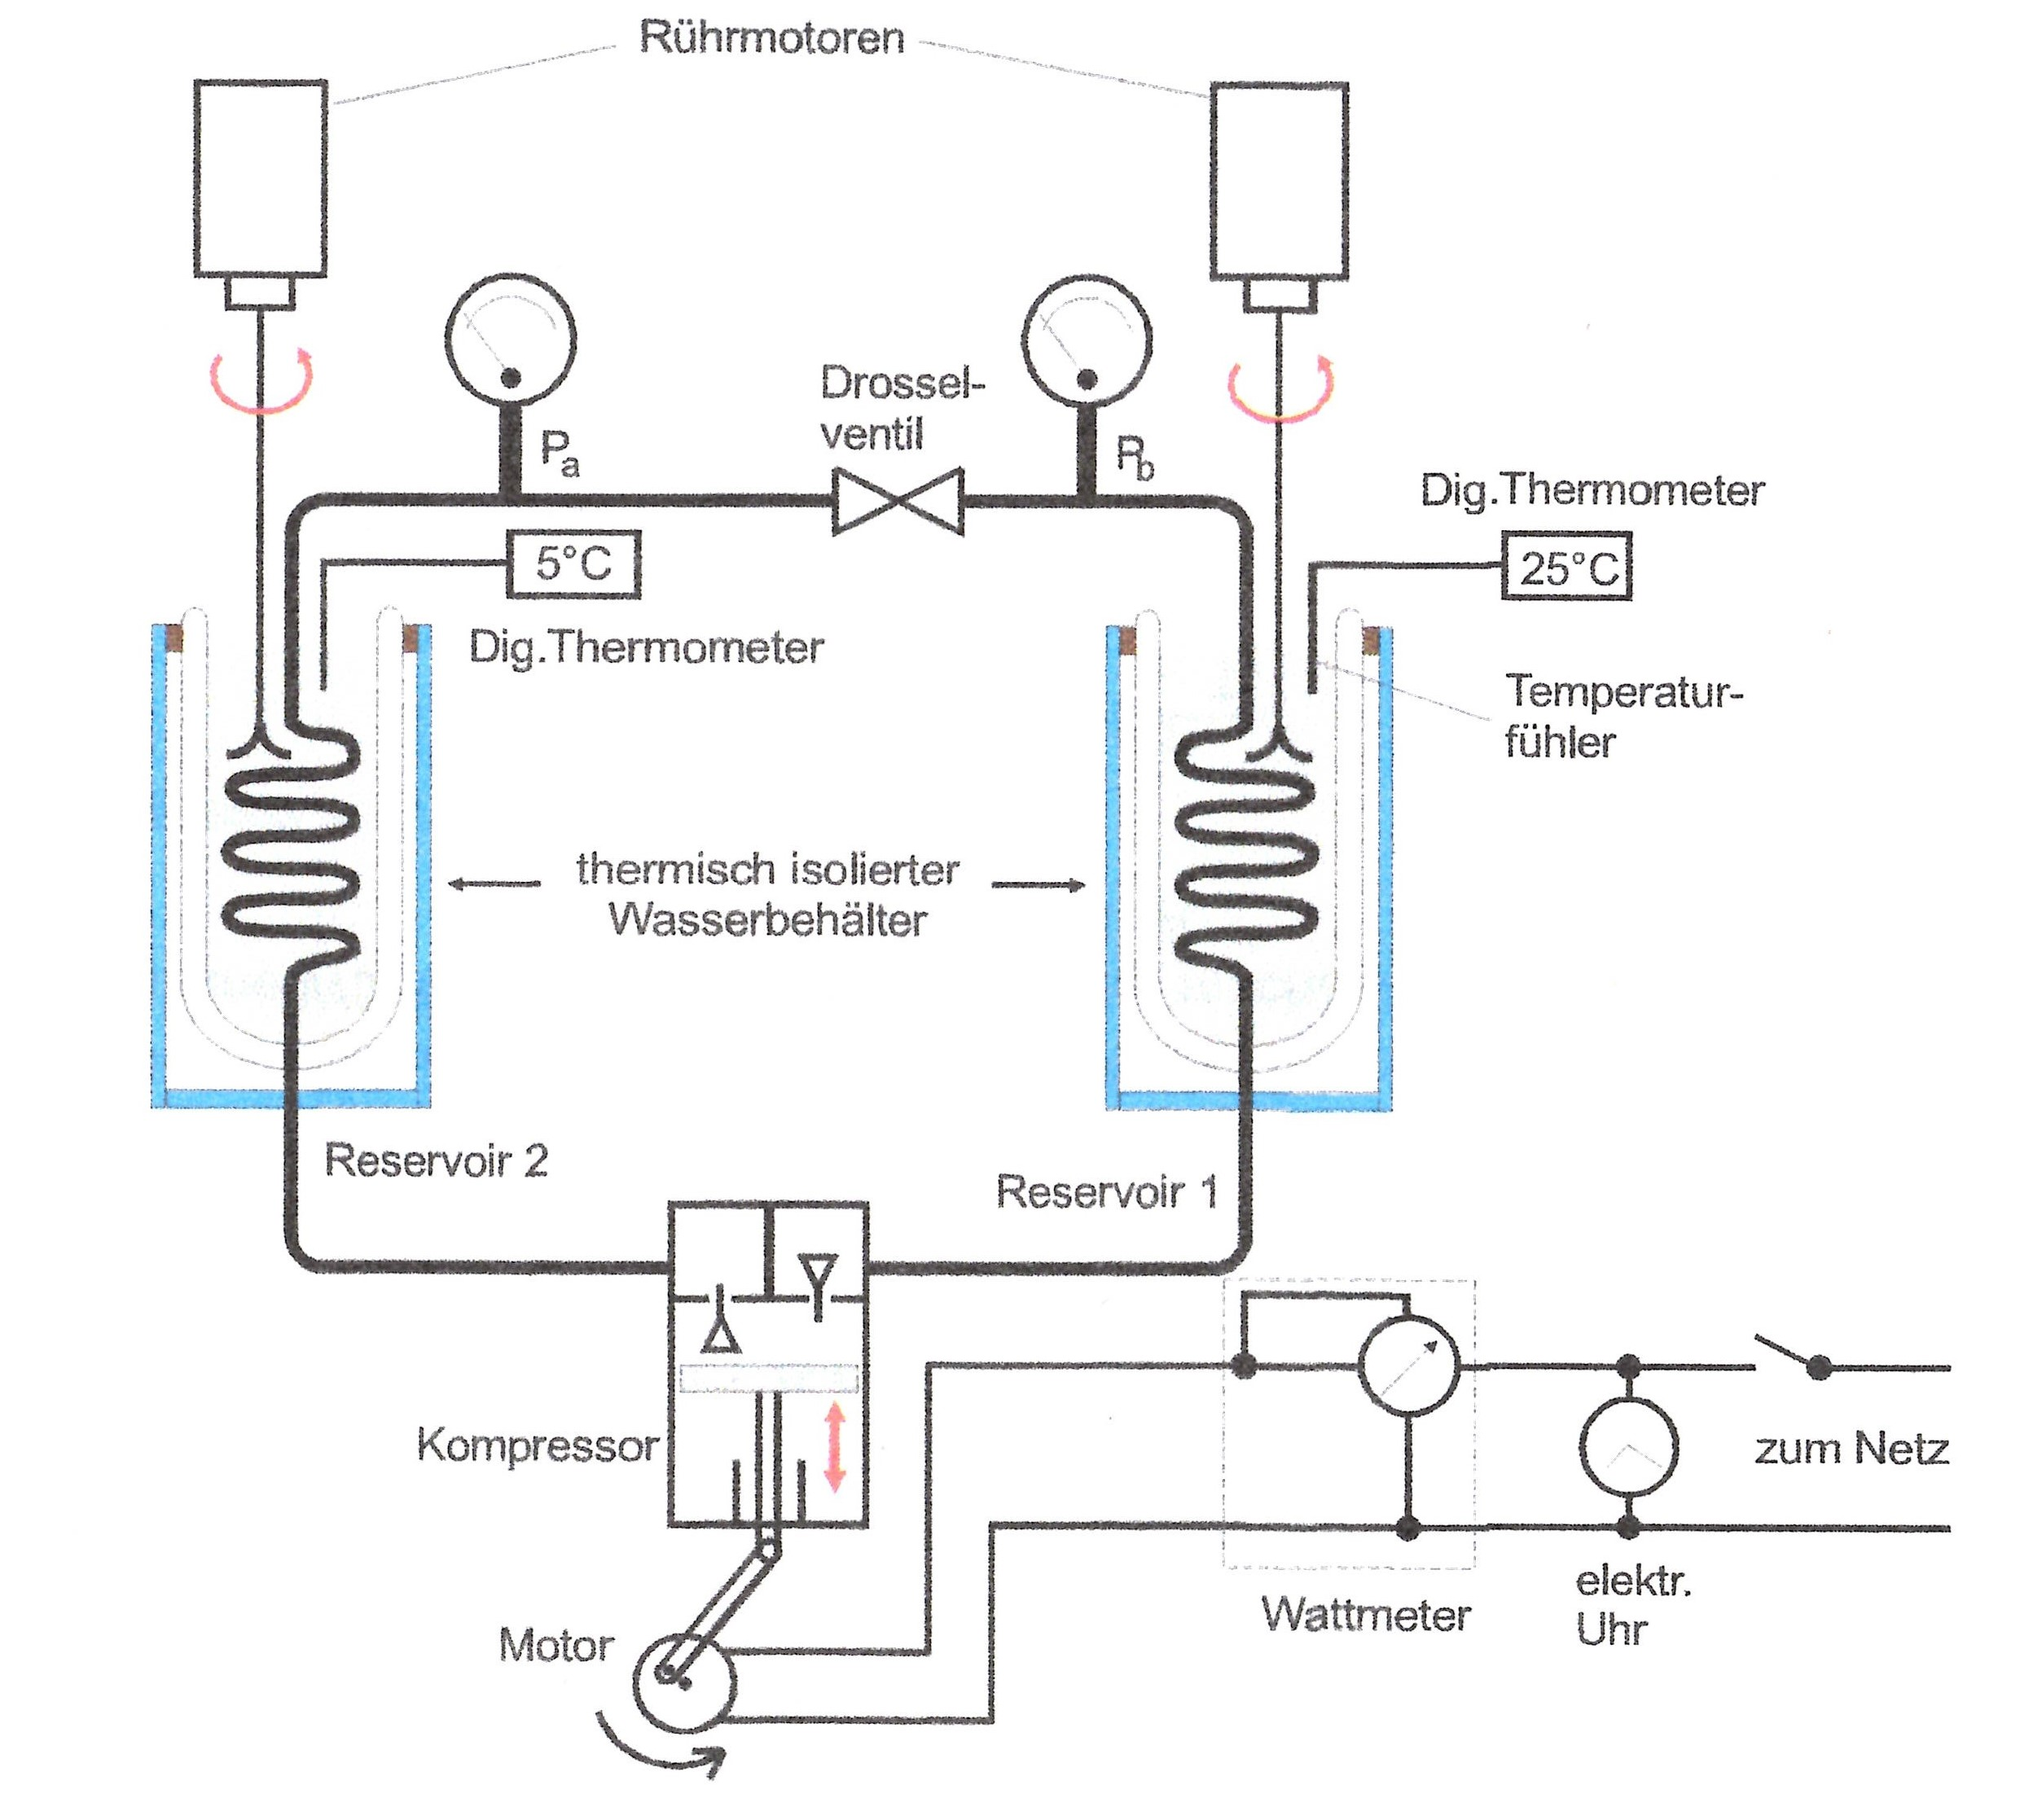
\includegraphics{Versuchs_Skizze.JPG}
  \caption{Versuchsaufbau}
  \label{fig:Aufbau}
\end{figure}

\subsection{Durchführung}

Am Anfang des Experimentes werden die beiden Reservoire mithilfe eines Messkolben mit $4 \mathup{l}$ Wasser befüllt. Nach Einbau der beiden Reservoire
in die Apparatur werden Rührstabe und Kompressor eingeschaltet. Um die beiden Reservoire optimal abzudichten, werden unter die beiden Behälter
noch Holzkeile geschoben. Nun werden im Abstand von einer Minute die verschiedenen Drücke und Temperaturen
von Reservoir 2 [$p_a, T_2$] und Reservoir 1 [$p_b, T_1$], sowie die durch den Kompressor eingebrachte Leistung $L$ gemessen und notiert. Bei dem Druck
wird dabei die innere schwarze Skala abgelesen und am Ende wird bei allen Werten noch $1 bar$ hinzuaddiert. Sobald
die Temperatur im Reservoir 2 die $50 °C$ Marke erreicht, wird der Kompressor wieder ausgeschaltet.

\newpage
\section{Auswertung}
In der Auswertung werden die gemessenen Temperaturen, Drücke und Leistungen als fehlerfrei angenommen.
\subsection{Temperaturverläufe}
Die während des Versuches gemessenen Temperaturen von Reservoir 1 und Reservoir 2 sind in dem Diagramm \ref{fig:Temperaturverlauf} dargestellt.
Die Temperatur in $\si{\kelvin}$ wurde gegenüber der Zeit in $\si{\second}$ aufgetragen.
\begin{figure}
  \centering
  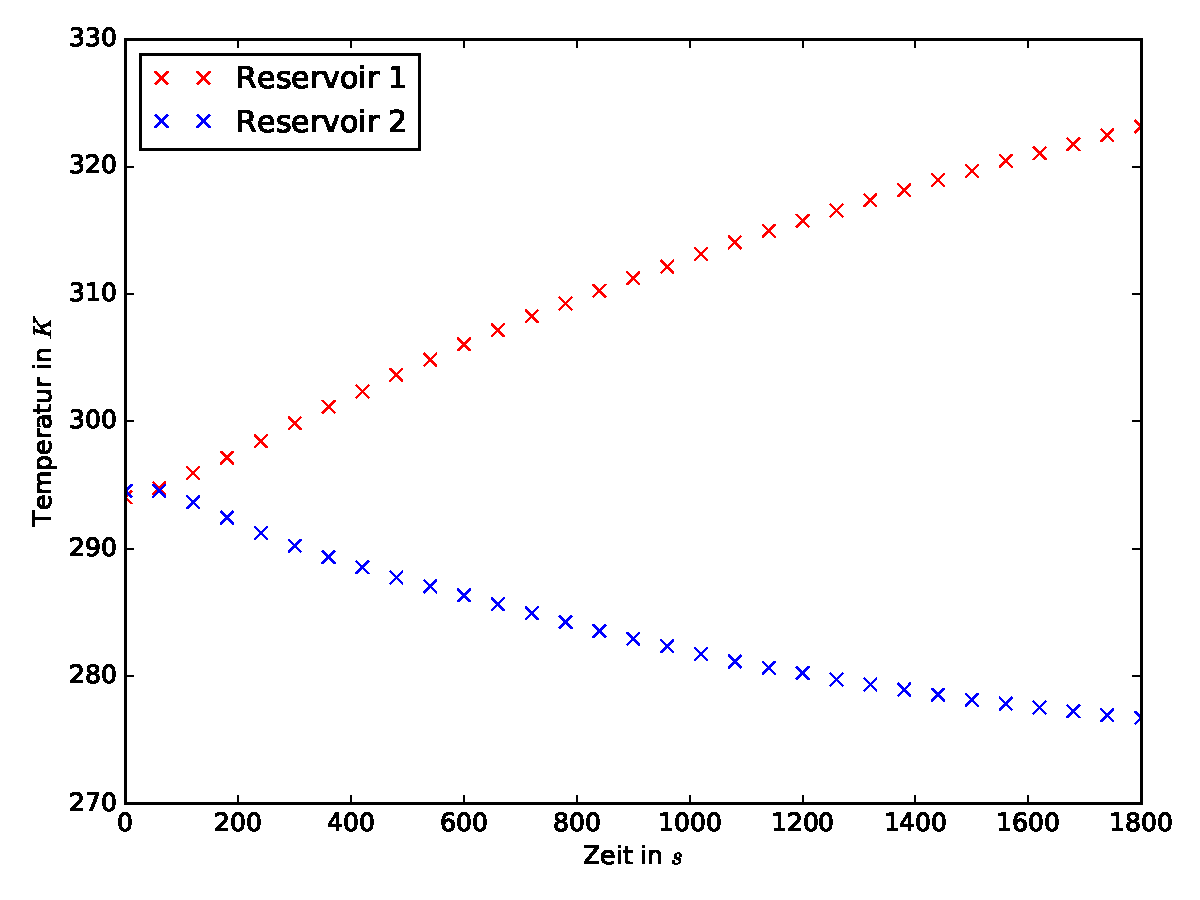
\includegraphics[width=\textwidth]{Temperatur_Zeit.pdf}
  \caption{Temperaturverlauf}
  \label{fig:Temperaturverlauf}
\end{figure}
\subsubsection{Ausgleichsfunktion}
Den Temperaturverlauf der beiden Reservoire wurde darüberhinaus durch eine nicht-lineare Ausgleichsrechnung dargestellt.
Hierfür wurde die quadratische Funktion $T(t) = A\cdot t^2 + B\cdot t + C$ verwendet. Der Fit wurde mit Hilfe von \textit{curve\_fit} erstellt, wobei die Fehler aus der Kovarianz-Matrix von \textit{curve\_fit} entstammen. An der Ausgleichskurve wird deutlich, dass sich die Temperaturveläufe relativ präzise approximieren lassen. Die Fehler sind in der selben Einheit, wie der zugehörige Parameterwerte.

\begin{figure}
  \centering
  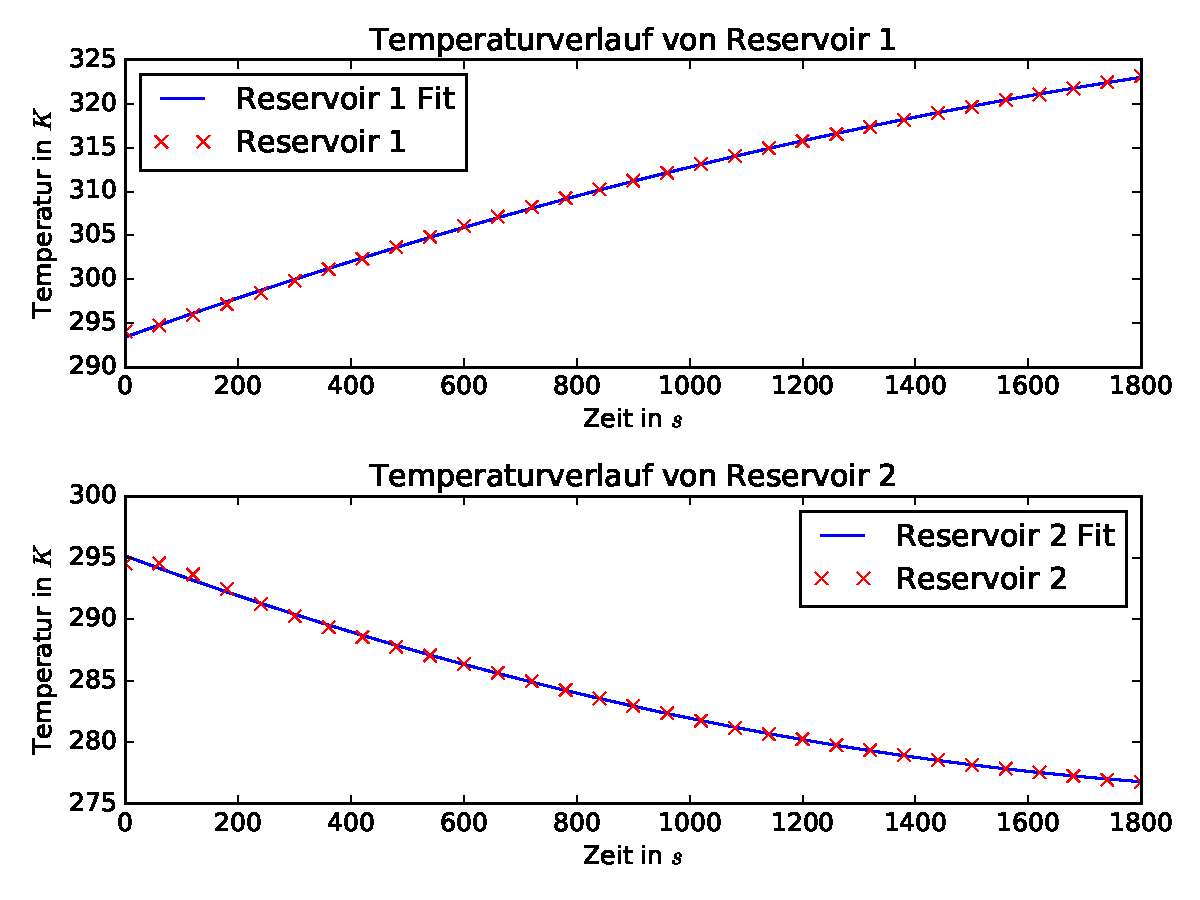
\includegraphics[width=\textwidth]{Temperatur_Zeit_Fit.pdf}
  \label{fig:Temperaturverlauf_Fit}
\end{figure}
\floatplacement{table}{htbp}
\begin{table}
   \centering
   \caption{Parameter der Ausgleichsrechnung}
   \label{tab:Ausgleichsrechnung}
   \begin{tabular}[width=0.4\textwidth]{S[table-format=1.0] S[table-format=1.3] S[table-format=1.3] S[table-format=1.4] S[table-format=1.5] S[table-format=2.3] S[table-format=1.4]}
       \toprule
       {\footnotesize{\emph{Reservoir}}}  & {\footnotesize{Parameter} $A$ \footnotesize{in} $\mu\frac{\si{\kelvin}}{\si{\second}^2}$} & {\footnotesize{\emph{Fehler}}} & {\footnotesize{Parameter} $B$ \footnotesize{in}  $\frac{\si{\kelvin}}{\si{\second}}$} & {\footnotesize{\emph{Fehler}}} & {\footnotesize{Parameter} $C$ \footnotesize{in} $\si{\kelvin}$} & {\footnotesize{\emph{Fehler}}} \\
       \midrule
       1 & -3,643 & 0,116 & 0,023 & 0,00022 & 29,343 & 0,0842 \\
       2 & 3,748 & 0,127 & -0,017 & 0,00024 & 29,515 & 0,0923 \\
       \bottomrule
   \end{tabular}
\end{table}
\FloatBarrier
\subsection{Differentialquotient der nicht-linearen Ausgleichsrechnung}
Der Differentialquotient $\frac{\mathup{d}}{\mathup{d}t} T(t)$ der Ausgleichskurve ergibt sich aus:
\begin{align*}
  \frac{\mathup{d}}{\mathup{d}t} T(t) = \frac{\mathup{d}}{\mathup{d}t}(A\cdot t^2 + b\cdot t + C) = 2 A\cdot t + B
\end{align*}
Der Differentialquotient wurde für die Zeiten $360 \si{\second}$, $720 \si{\second}$, $1080 \si{\second}$ und $1440 \si{\second}$ berechnet.
Daraus ergeben sich die Werte:
\begin{align*}
  \frac{\mathup{d}}{\mathup{d}t} T_1(360) &= (0,0204 \pm 0,00023) \frac{\si{\kelvin}}{\si{\second}} &
  \frac{\mathup{d}}{\mathup{d}t} T_2(360) &= (-0,0143 \pm 0,00025) \frac{\si{\kelvin}}{\si{\second}} \\
  \frac{\mathup{d}}{\mathup{d}t} T_1(720) &= (0,0177 \pm 0,00027) \frac{\si{\kelvin}}{\si{\second}} &
  \frac{\mathup{d}}{\mathup{d}t} T_2(720) &= (0,0177 \pm 0,00030) \frac{\si{\kelvin}}{\si{\second}} \\
  \frac{\mathup{d}}{\mathup{d}t} T_1(1080) &= (0,151 \pm 0,00033) \frac{\si{\kelvin}}{\si{\second}} &
  \frac{\mathup{d}}{\mathup{d}t} T_2(1080) &= (0,151 \pm 0,00036) \frac{\si{\kelvin}}{\si{\second}} \\
  \frac{\mathup{d}}{\mathup{d}t} T_1(1440) &= (0,0125 \pm 0,00040) \frac{\si{\kelvin}}{\si{\second}} &
  \frac{\mathup{d}}{\mathup{d}t} T_2(1440) &= (0,0125 \pm 0,00044) \frac{\si{\kelvin}}{\si{\second}}
\end{align*}
Die Fehler werden nach der Gaußschen Fehlerfortpflanzung wie folgt ermittelt:
\begin{align*}
  \increment\frac{\mathup{d}}{\mathup{d}t} T(t) = \sqrt{\left(\frac{\mathup{d^2}T(t)}{\mathup{d}tA}\cdot\increment A\right)^2 + \left(\frac{\mathup{d^2}T(t)}{\mathup{d}tB}\cdot\increment B\right)^2}
\end{align*}
Dabei ist $\increment x$ jeweils der Fehler des hinterstehenden Parameters.
\subsection{Bestimmug der Güteziffer \texorpdfstring{$\nu$}{z}}
In dem folgendem Abschnitt wird die Gütteziffer $\nu$ der verwendeten Wärmepumpe bestimmt. Diese ergibt sich aus der Formel \eqref{eqn:Güte_theo}. Für die Wärmekapazität der Apparatur wurde der Wert $750 \frac{\si{\joule}}{\si{\kelvin}}$ verwendet. Dieser war an dem Versuchsaufbaus angegeben. Die Wärmekapazität des Wassers ist für einen Liter mit $4182\frac{\si{\joule}}{\si{\kelvin}}$ zu bemessen. In dem Versuch wurden die Reservoire mit $4 \mathup{l}$ Wasser befüllt.
Mit der Ausgleichgeraden ergibt sich für $\nu$ die Formel:
\begin{equation}
  \label{eqn:Güte}
  \nu = \frac{1}{N}(m_1c_{\omega} + m_kc_k)(2 A\cdot t + B)
\end{equation}
In der Formel \eqref{eqn:Güte} sind die Parameter $A$ und $B$ die einzigen fehlerbehafteten Größen.
\floatplacement{table}{htbp}
\begin{table}
   \centering
   \caption{Güteziffer}
   \label{tab:Güteziffer}
   \begin{tabular}[width=0.4\textwidth]{S[table-format=3.0] S[table-format=1.3] S[table-format=1.4] S[table-format=2.3]}
       \toprule
       {\emph{Zeit} in \si{\second}} & {$\nu_{\tiny{real}}$} & {\emph{Fehler}} & {$\nu_{\tiny{ideal}}$} \\
       \midrule
       360 & 2,826 & 0,0322 & 25,521 \\
       720 & 2,564 & 0,0395 & 13,230 \\
       1080 & 2,115 & 0,0464 & 9,546 \\
       1440 & 1,748 & 0,0557 & 7,895 \\
       \bottomrule
   \end{tabular}
\end{table}
Die Fehler wurden mit Hilfe der Gaußschen Fehlerfortpflanzung berechnet.

Da nur $A$ und $B$ mit Fehlern behaftet sind ergibt sich die folgende Fehlerformel.
\begin{align*}
  \increment\nu = \sqrt{\left(\frac{\mathup{d\nu}}{\mathup{dA}}\increment A\right)^2+ \left(\frac{\mathup{d\nu}}{\mathup{dB}}\increment B\right)^2}
\end{align*}
Die ideale Güteziffer ist fehlerfrei, da sie über die Temperaturen errechnet wurde. Diese ergibt sich aus Formel \eqref{eqn:A1.2}.
\subsection{Bestimmung des Massendurchsatzes}
Damit der Massedurchsatz bestimmt werden kann, muss zunächst die Verdampfungswärme $L$ ermittelt werden. Die Verdampfungswärme ist über $L = R\cdot T \log(\frac{p_0}{p})$ zu berechnen. Dabei ist $R$ die allgemeine Gaskonstante, $T$ die momentane Temperatur, $p_0$ der Anfangswert des Druckes und $p$ der momentane Druck ist. In dem folgendem Diagramm sind die $\log(\frac{p_0}{p})$ gegenüber den reziproken Temperaturen aufgetragen.
\floatplacement{figure}{htbp}
\begin{figure}
  \centering
  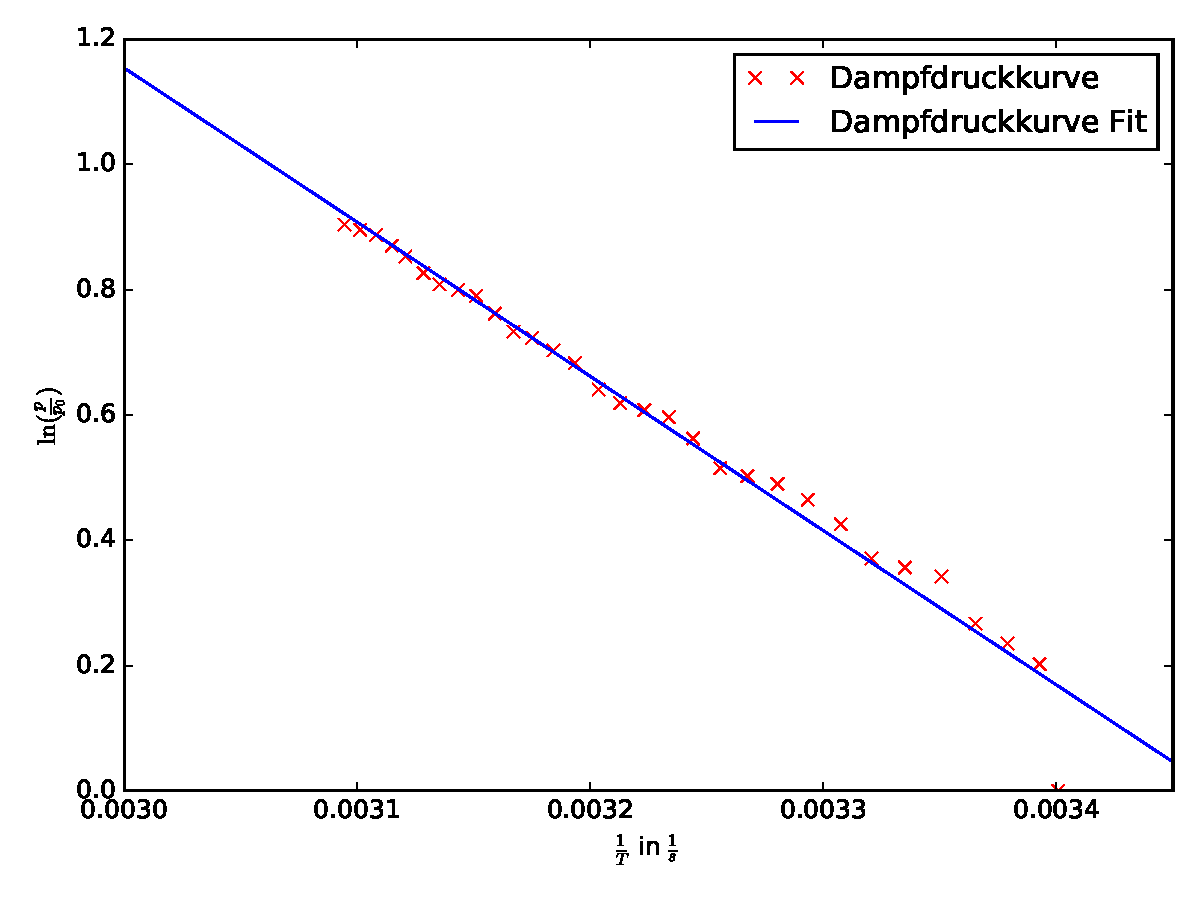
\includegraphics[width=\textwidth]{Massendurchsatz.pdf}
  \label{fig:Dampfdruckkurve}
  \subcaption{Graph zur Bestimmung der Verdampfungswärme}
\end{figure}

Die Ausgleichsgerade ergibt sich aus der Steigung $m = -2462,019$ und dem Achsenabschnitt $n = 8,540$. Die Ausgleichsrechnung wurde mit Hilfe von \textit{curve\_fit} bewerkstelligt. Die Parameter $m$ und $n$ sind mit den Fehlern $\increment m = 68,222$ und $\increment n = 0.220$ behaftet. Aus der Steigung $m$ und der allgemeinen Gaskonstanten $R$ lässt sich die Verdampfungswärne über $L = -mR$ errechnen.
Somit ergibt sich für die Verdampfungswärme schließlich $L = (20470,715 \pm 567,230) \frac{\si{\joule}\si{\second}}{\si{\mol}\si{\kelvin}}$.
Mit $L$ lässt sich nun auch der Massendurchsatz nach \eqref{eqn:Massendurchsatz1} berechnen.
\floatplacement{table}{htbp}
\begin{table}
   \centering
   \caption{Massendurchsatz}
   \label{tab:Massendurchsatz}
   \begin{tabular}[width=0.4\textwidth]{S[table-format=3.0] S[table-format=1.5] S[table-format=1.5]}
       \toprule
       {\emph{Zeit} in \si{\second}} & {$\frac{\mathup{d}m}{\mathup{d}t}$ in $\frac{\si{\mol}}{\si{\second}}$} & {\emph{Fehler}} \\
       \midrule
       360 & -0,01217 & 0,00043 \\
       720 & -0,00987 & 0,00042 \\
       1080 & -0,00756 & 0,00044 \\
       1440 & -0,00526 & 0,00046 \\
       \bottomrule
   \end{tabular}
\end{table}

Die Fehler ergeben sich mit Hilfe der Gaußschen Fehlerfortpflanzung wie folgt.
\begin{align*}
  \increment\frac{\mathup{d}m}{\mathup{d}t} = \sqrt{\left(\frac{\mathup{d^2}m}{\mathup{d}tA}\cdot\increment A\right)^2 + \left(\frac{\mathup{d^2}m}{\mathup{d}tB}\cdot\increment B\right)^2 + \left(\frac{\mathup{d^2}m}{\mathup{d}tL}\cdot\increment L\right)^2}
\end{align*}
\subsection{Bestimmung der mechanische Kompressorleistung \texorpdfstring{$N_{mech}$}{t}}
Wie in der Theorie erwähnt wurde, wird der natürliche Wärmeenergiefluss mit Hilfe von mechanischer Arbeit umgekehrt.
Die dafür benötigte Leistung $N_{mech}$ lässt sich über \eqref{eqn:Nmech} berechnen. Vorerst muss der Massendurchsatz von $\frac{\si{\mol}}{\si{\second}}$ in die Einheiten $\frac{\si{g}}{\si{\mol\second}}$ umgerechnet werden, sodass die mechanische Leistung in $\si{\watt}$ errechnet wird. Das verwendete Gas Dichlordiflourmethan ($\ce{Cl2F2C}$)hat eine Molare Masse von $120,91 \frac{\si{\g}}{\si{\mol}}$.
Die Dichte $\rho$ lässt sich unter der Annahme, dass der Kompressor adiabatisch arbeitet über die ideale Gasgleichung festlegen.
\begin{equation*}
  p V = n R T \quad\iff\quad n R = \frac{p V}{T}
\end{equation*}
Darausfolgt für $n_0R = n_2R$, mit $V = \frac{m}{\rho}$:
\begin{equation*}
  \frac{p_0m}{\rho_0T_0} = \frac{p_2m}{\rho T_2} \quad\iff\quad\frac{p_0}{\rho_0T_0} = \frac{p_2}{\rho T_2}
  \quad\iff\quad\rho = \frac{p_2\rho_0T_0}{p_0T_2}
\end{equation*}
Als Werte waren $\rho_0 = 5,51 \frac{\si{g}}{\si{l}}$ bei $T = 273,15 \si{\kelvin}$, $p_0 = 1 \si{bar}$ und $\kappa = 1,14$ vorgegeben.
Durch \eqref{eqn:Nmech} ergeben sich die in Tabelle \ref{tab:Nmech} visualisierten Werte.
\floatplacement{table}{htbp}
\begin{table}
   \centering
   \caption{Mechanische Kompressorleistung $N_{mech}$ und Dichte $\rho$}
   \label{tab:Nmech}
   \begin{tabular}[width=0.4\textwidth]{S[table-format=3.0] S[table-format=2.3] S[table-format=1.4] S[table-format=1.5]}
       \toprule
       {\emph{Zeit} in $\si{\second}$} & {\emph{Dichte} $\rho$ in $\frac{\si{g}}{\si{\meter}^3}$} & {\emph{Leistung} $N_{mech}$ in $\si{\watt}$} & {\emph{Fehler}} \\
       \midrule
       360 & 24,447 & 0,1029 & 0.00356 \\
       720 & 21,655 & 0,1027 & 0.00430 \\
       1080 & 20,342 & 0,0911 & 0.00510 \\
       1440 & 19,451 & 0,0705 & 0.00603 \\
       \bottomrule
   \end{tabular}
\end{table}
Der Fehler für die mechanische Leistung $N_{mech}$ ergibt sich aus der Gaußschen Fehlerfortpflanzung wie folgt.
\begin{align*}
  \increment N_{mech} = \sqrt{\left(\frac{\mathup{d}N_{mech}}{\mathup{d}\frac{\mathup{d}m}{\mathup{d}t}}\cdot\increment\frac{\mathup{d}m}{\mathup{d}t}\right)^2}
\end{align*}
\section{Diskussion}
Im Folgendem werden die Versuchsergebnisse diskutiert. Dabei wird besonders auf den Vergleich zwischen der idealen Güteziffer $\nu_{ideal}$ und der empirisch gefundenen Güteziffer $\nu_{real}$ eingegangen.
In dem Versuch wird deutlich, dass sich die Temperaturverläufe geeignet durch ein quadratisches Polynom approximieren lassen. Anhand der Ausgleichsrechnung wurde dies deutlich. Die Messwerte weichen lediglich minimal von dem Graphen der Ausgleichskurve ab.
Die beiden Güteziffern unterscheiden sich deutlich. Gründe dafür könnte die idealisierte Annahme sein, dass der Kompressor adiabatisch arbeitet. Zudem waren die Reservoire nicht optimal isoliert, sodass ein Wärmeaustausch mit der Umgebung stattgefunden hat. Dadurch wird die Güte der Wärmepumpe vermindert, weil mehr Arbeit aufgewendet werde muss, um den Wärmeenergieverlust auszugleichen. Desweiteren waren die Skalierungen an den Messapperaturen nicht fein genug dargestellt, um die zweite Nachkommastelle bei den Manometern genau ablesen zukönnen. Daher wurden alle verwendeten Drücke auf die zweite Nachkommastelle gerundet und sind so in Tabelle \ref{tab:Messdaten} dargestellt. Ebenso grob war die Skalierung auf dem Generator des Kompressors, sodass die abgelesene Leistung ohne Nachkommastellen angegeben wurde. Die Thermometer, mit denen die Temperatur in den Reservoiren gemessen wurde, waren digital und erlaubten eine genaue Messung bis auf die zweite Nachkommastelle. Es wird deutlich, dass die Messbedingungen nicht optimal waren, sodass die Güte der Wärmepumpe bereits dadurch gemindert wurde. Die gemachten Messfehler und die nicht erfüllbaren idealisierten Annahmen führen somit dazu, dass die realen Werte deutlich von den theoretischen Werten Abweichen.
\newpage
\FloatBarrier
\section{Messdaten}
\floatplacement{table}{htbp}
\begin{table}
   \small
   \centering
   \caption{Messdaten}
   \label{tab:Messdaten}
   \begin{tabular}{S[table-format=3.0] S[table-format=1.1] S[table-format=1.1] S[table-format=1.2] S[table-format=1.2] S[table-format=3.0]}
       \toprule
       {\emph{Zeit} in $\si{\second}$} & {$T_1$ in $\si{\kelvin}$} & {$T_2$ in $\si{\kelvin}$} & {$p_1$ in $\si{bar}$} & {$p_2$ in $\si{bar}$} & {\emph{Leistung} in $\si{W}$} \\
       \midrule
       0 & 294.05 & 294.55 & 4.9 & 5.0 & 0 \\
       60 & 294.75 & 294.55 & 6.0 & 4.3 & 115 \\
       120 & 295.95 & 293.65 & 6.2 & 4.6 & 120 \\
       180 & 297.15 & 292.45 & 6.4 & 4.7 & 125 \\
       240 & 298.45 & 291.25 & 6.9 & 4.8 & 125 \\
       300 & 299.85 & 290.25 & 7.0 & 4.8 & 127 \\
       360 & 301.15 & 289.35 & 7.1 & 4.7 & 126 \\
       420 & 302.35 & 288.55 & 7.5 & 4.6 & 125 \\
       480 & 303.65 & 287.75 & 7.8 & 4.5 & 124 \\
       540 & 304.85 & 287.05 & 8.0 & 4.4 & 123 \\
       600 & 306.05 & 286.35 & 8.1 & 4.3 & 123 \\
       660 & 307.15 & 285.65 & 8.2 & 4.2 & 122 \\
       720 & 308.25 & 284.95 & 8.6 & 4.1 & 121 \\
       780 & 309.25 & 284.25 & 8.9 & 4.0 & 121 \\
       840 & 310.25 & 283.55 & 9.0 & 4.0 & 122 \\
       900 & 311.25 & 282.95 & 9.1 & 3.9 & 122 \\
       960 & 312.15 & 282.35 & 9.3 & 3.8 & 123 \\
       1020 & 313.15 & 281.75 & 9.7 & 3.8 & 124 \\
       1080 & 314.05 & 281.15 & 9.9 & 3.8 & 125 \\
       1140 & 314.95 & 280.65 & 10.1 & 3.7 & 125 \\
       1200 & 315.75 & 280.25 & 10.2 & 3.7 & 125 \\
       1260 & 316.55 & 279.75 & 10.5 & 3.6 & 125 \\
       1320 & 317.35 & 279.35 & 10.8 & 3.6 & 125 \\
       1380 & 318.15 & 278.95 & 10.9 & 3.6 & 125 \\
       1440 & 318.95 & 278.55 & 11.0 & 3.6 & 125 \\
       1500 & 319.65 & 278.15 & 11.2 & 3.6 & 125 \\
       1560 & 320.45 & 277.85 & 11.5 & 3.5 & 125 \\
       1620 & 321.05 & 277.55 & 11.7 & 3.5 & 125 \\
       1680 & 321.75 & 277.25 & 11.9 & 3.5 & 125 \\
       1740 & 322.45 & 276.95 & 12.0 & 3.5 & 125 \\
       1800 & 323.15 & 276.75 & 12.1 & 3.4 & 125 \\
      \bottomrule
  \end{tabular}
\end{table}
Mit $T_1$ der Temperatur aus Reservoir 1, $T_2$ der Temperatur aus Reservoir 2, $p_1$ dem Druck aus Reservoir 1 und $p_2$ dem Druck aus Reservoir 2.
\end{document}
